\documentclass[a4paper,11pt,oneside]{article}

\usepackage[utf8]{inputenc}
\usepackage[T1]{fontenc}
\usepackage[ngerman]{babel}
\usepackage{amssymb}
\usepackage{amsmath}
\usepackage{amsthm}
\usepackage{graphicx}
\usepackage{float}
\usepackage{hyperref}
\usepackage{bm}
\usepackage[most]{tcolorbox}
\usepackage[top=2cm, bottom=2.5cm, right=2.5cm, left=2.5cm]{geometry}

\newtheorem{theorem}{Satz}
\theoremstyle{definition}
\newtheorem{definition}{Definition}
\newtheorem{remark}{Bemerkung}
\newtheorem{example}{Beispiel}
\hypersetup{colorlinks=true,urlcolor=blue,linkcolor=blue}
\renewcommand{\familydefault}{\sfdefault}
\parindent0pt
\parskip6pt
\def\GB#1{\colorbox{gray!30}{#1}}
\def\RM#1{\uppercase\expandafter{\romannumeral #1\relax}}
\def\OP#1{\textcolor{blue}{(\textnormal{\textrm{\textsc{#1}})}}}

\begin{document}

\title{Lösungsverfahren für lineare Gleichungssysteme\\\vskip0.5em\small (Basierend auf dem Skript ,,Mathematik II für Studierende der BWL, Chemie und anderer Studiengänge'' von Prof.~Dr.~Michael~Kolonko)}
\author{Michael Kolonko, Alexander Herzog\\\href{mailto:alexander.herzog@tu-clausthal.de}{\small\texttt{alexander.herzog@tu-clausthal.de}}\\\href{https://a-herzog.github.io/LGSSolver/}{\small\texttt{a-herzog.github.io/LGSSolver}}}
\date{}

\maketitle



\section{Fragestellung und Definitionen}

\begin{example}\label{Bsp:RosenNelken}
Ein Gärtner hat $b_1:=500$ m$^2$ Land zur Bepflanzung mit Tulpen, Rosen und Nelken zur Verfügung. Das Saatgut kostet ihn (pro m$^2$)
\begin{eqnarray*}
a_{21}&:=&3\quad \text{Euro (Tulpen)},\\
a_{22}&:=&7\quad \text{Euro (Rosen) und}\\
a_{23}&:=&5\quad \text{Euro (Nelken).}
\end{eqnarray*}
Er hat insgesamt $b_2=3000$ Euro zur Verfügung. Außerdem möchte er seine Bestände an Düngemitteln aufbrauchen. Von Düngemittel I hat er $b_3:=890$ kg und von Düngemittel II $b_4:=1000$ kg. Die Pflanzen brauchen seiner Meinung nach pro m$^2$
\begin{equation*}
\begin{alignedat}{3}
a_{31}&:=1\quad\text{kg (Tulpen),}&a_{41}&:=2&&\text{kg}\\
a_{32}&:=2\quad\text{kg (Rosen)\quad von Mittel I\quad bzw.\quad }&a_{42}&:=2&&\text{kg\quad von Mittel II.}\\
a_{33}&:=3 \quad\text{kg (Nelken)}&a_{43}&:=2&&\text{kg}
\end{alignedat}
\end{equation*}
Wieviel m$^2$ Tulpen, Rosen, Nelken sollten angepflanzt werden?

Setzt man $x_1$ für die Anzahl an m$^2,$ die mit Tulpen bepflanzt werden sollen, $x_2$ für die mit Rosen und $x_3$ für die mit Nelken, so ergibt der Text oben, dass $x_1$, $x_2$ und $x_3$ gesucht sind, die folgendes Gleichungssystem erfüllen:

\begin{alignat}{2}\label{eq:RosenNelken}
x_1+\ \ x_2+\ \ x_3&=500&&(\text{Fläche}) \cr
3x_1+7x_2+5x_3&=3000&&(\text{Euro})\cr
x_1+2x_2+3x_3&=890&\qquad&(\text{Düngemittel I})\cr
2x_1+2x_2+2x_3&=1000&&(\text{Düngemittel II})
\end{alignat}
oder kürzer
\begin{eqnarray*}
a_{11}x_1+a_{12}x_2+a_{13}x_3&=b_1\cr a_{21}x_1+a_{22}x_2+a_{23}x_3&=b_2\cr a_{31}x_1+a_{32}x_2+a_{33}x_3&=b_3\cr
a_{41}x_1+a_{42}x_2+a_{43}x_3&=b_4\cr
\end{eqnarray*}
bzw.
$$
Ax=b
$$
mit den Bezeichnungen
$$
A:=
\begin{pmatrix}
a_{11}&a_{12}&a_{13}\cr
a_{21}&a_{22}&a_{23}\cr
a_{31}&a_{32}&a_{33}\cr
a_{41}&a_{42}&a_{43}\cr
\end{pmatrix}
:=
\begin{pmatrix}
1&1&1\cr
3&7&5\cr
1&2&3\cr
2&2&2\cr
\end{pmatrix}
,\qquad
b:=
\begin{pmatrix}
b_1\cr
b_2\cr
b_3\cr
b_4\cr
\end{pmatrix}
:=
\begin{pmatrix}
500\cr
3000\cr
890\cr
1000
\end{pmatrix}
\quad \text{und} \quad
x:=\begin{pmatrix}
x_1\cr
x_2\cr
x_3\cr
\end{pmatrix}
.
$$
Gesucht ist also eine Lösung $x\in\mathbb R^3$ des linearen Gleichungssystems $Ax=b$ zu gegebenem (d.\,h.\ bekanntem) $A\in\mathbb R^{4\times 3}$ (eine $ (4\times 3)$-Matrix) und $b\in\mathbb R^4$.
\end{example}

Bei der Untersuchung von (linearen) Gleichungssystemen $ Ax=b$ mit gegebenem $A$ und $b$ stellen sich ganz allgemein die folgenden Fragen:

\paragraph{1.\ Existenz einer Lösung:}~\\
Gibt es ein $x\in\mathbb R^3$, das $Ax=b$ erfüllt?

Z.\,B.\ erfüllt $x:=\begin{pmatrix}120\cr 370\cr 10\end{pmatrix}$ das Gleichungssystem \eqref{eq:RosenNelken} aus Beispiel \ref{Bsp:RosenNelken}, ändert man aber die dritte Zeile von $A$ (die Aussagen über den Bedarf an Düngemittel I trifft) etwa zu $a_{31}=a_{32}=a_{33}:=1,$ so gibt es \emph{keine} Lösung.

\paragraph{2.\ Eindeutigkeit der Lösung:}~\\
Gibt es mehrere $x\in\mathbb R^3$, die $Ax=b$ erfüllen?

Für $a_{31}=a_{32}=a_{33}:=1$ und $b_3:=500$ z.\,B.\ ist $x=\begin{pmatrix}125-0{,}5\lambda \cr 375-0{,}5\lambda \cr \lambda \end{pmatrix}$ für jedes $\lambda\in\mathbb R$ eine Lösung von \eqref{eq:RosenNelken}.

\textbf{3.\ Lösungsverfahren:}~\\
Wie kann zu gegebenen $A$ und $b$ eine Lösung $x$ zu $ Ax=b$ praktisch (algorithmisch) gefunden werden? Z.\,B.\ durch sukzessives Einsetzen (s.u.).

\begin{definition}\label{Def:LGS}
Gegeben seien $A:=(a_{ij})_{1\le i\le m,\ 1\le j\le n}$, $a_{ij}\in\mathbb R$, $m,n\in\mathbb N$, eine $(m\times n)$-Matrix und $b:=\begin{pmatrix}b_1\cr\vdots\cr b_m\end{pmatrix}\in\mathbb R^m$.
\begin{enumerate}
\item
Das Schema
$$
\begin{alignedat}{4}
a_{11}x_1&\ +\ &a_{12}x_2&\ +\ & \cdots &\ +\ &a_{1n}x_n &=b_1\\
a_{21}x_1&\ +\ &a_{22}x_2&\ +\ & \cdots &\ +\ &a_{2n}x_n &=b_2\\
\vdots &&\vdots &&&&\vdots&\cr
a_{m1}x_1&\ +\ &a_{m2}x_2&\ +\ & \cdots &\ +\ &a_{mn}x_n &=b_m
\end{alignedat}
$$
bzw.
$$
\sum _{j=1}^n a_{ij}x_j=b_i\qquad \text{für alle}~ 1\leq i\leq m
$$
oder kurz
$$
Ax=b
$$
nennt man ein \emph{lineares Gleichungssystem} (LGS) mit $m\in\mathbb N$ Gleichungen in $n\in\mathbb N$ \emph{Unbekannten} $x_1,\ldots,x_n$. $A$ heißt die \emph{Koeffizientenmatrix}, ein Vektor $x\in\mathbb R^n$ mit $Ax=b$ heißt eine \emph{Lösung} des Gleichungssystems. Mit
$$
{\mathbb L}:=\{x\in\mathbb R^n\mid Ax=b\}
$$
bezeichnen wir die \emph{Lösungsmenge}.
\item
Gilt $b=0$, so heißt das LGS \emph{homogen}, für $b\ne0$ \emph{inhomogen}.
\item
Die Matrix
$$
(A\mid b)
:=\left(\begin{array}{ccc|c}
a_{11}&\ldots& a_{1n}& b_1\\
a_{21}&\ldots&a_{2n}& b_2\\
\vdots &&\vdots &\vdots \\
a_{k1}&\ldots &a_{kn}& b_k
\end{array}\right)
$$
heißt die \emph{erweiterte Koeffizientenmatrix} des LGS.
\end{enumerate}
\end{definition}

Tauchen in dem Gleichungssystem negative Ausdrücke auf, so wird das ,,$-$'' als Vorzeichen an dem entsprechenden Koeffizienten behandelt. Fehlt in einer Gleichung eine Unbekannte, so wird der entsprechende Koeffizient $=0$ gesetzt, also z.\,B.
$$
\begin{aligned}
3x_1&\ -\ &7x_2&\ +\ &5x_3&=3000 \\
x_1&\ +\ &&\ \ &3x_3&=-890 \\
-2x_1&\ +\ &2x_2&\ \ &&=0
\end{aligned}
\qquad\text{mit}\qquad (A\mid b)
:=\left(\begin{array}{ccc|c}
3&-7& 5& 3000\\
1&0&3& -890\\
-2&2 &0& 0
\end{array}\right).
$$



\section{Lösungsverfahren}

Wir betrachten ein LGS $ Ax=b $ mit gegebener $(m\times n)$-Matrix $A$ und ,,rechter Seite'' $b\in\mathbb R^m$. $x=(x_1 ,\ldots, x_n)^T\in\mathbb R^n$ seien die (gesuchten) Unbekannten. Als Beispiel kann das LGS aus \eqref{Bsp:RosenNelken} gelten
\begin{alignat}{4}
x_1&\ +\ &x_2&\ +\ &x_3&=500 \tag{\RM{1}}\\
3x_1&\ +\ &7x_2&\ +\ &5x_3&=3000 \tag{\RM{2}}\\
x_1&\ +\ &2x_2&\ +\ &3x_3&=890 \tag{\RM{3}}\\
2x_1&\ +\ &2x_2&\ +\ &2x_3&=1000 \tag{\RM{4}}
\end{alignat}
Dabei werden die Gleichungen zur leichteren Bezugnahme manchmal mit römischen Zahlen durchnummeriert. Für die erweiterte Koeffizientenmatrix gilt hier
$$
(A\mid b)=\left(\begin{array}{ccc|c}
1&1&1&500\\
3&7&5&3000\\
1&2&3&890\\
2&2&2&1000
\end{array}\right).
$$
Der senkrechte Strich wird manchmal auch weggelassen, er soll andeuten, dass die letzte Spalte eine Sonderrolle spielt.

Die Matrix $(A\mid b)$ enthält alle Information aus dem ursprünglichen Gleichungssystem $ Ax=b$. Dabei entsprechen die $m$ Zeilen den Gleichungen, den ersten $n$ Spalten werden die Unbekannten $x_1,\ldots,x_n$ zugeordnet, die $(n+1)$-te Spalte ist die rechte Seite des LGS. Zur Lösung des LGS, d.\,h.\ zur Feststellung, ob es lösbar ist und wie gegebenenfalls die Menge $\mathbb L$ der Lösungen aussieht, genügt es daher, die erweiterte Koeffizientenmatrix zu untersuchen.

Diese Matrix kann durch  Vertauschungen und einfache lineare Operationen so verändert werden, dass die Lösbarkeit und die Menge $\mathbb L$ unmittelbar aus der Matrix abgelesen werden können. Wir benutzen die folgenden Operationen für $(A\mid b)$:

\begin{center}\fboxsep0.5ex
\framebox{\parbox[t]{14cm}{
\begin{enumerate}
\item
\OP{Ver}: Vertauschen zweier Zeilen,
\item
\OP{Mul}: Multiplikation einer Zeile mit einer Konstanten,
\item
\OP{Add}: Hinzuaddieren des Vielfachen einer Zeile zu einer anderen Zeile,
\item
\OP{Spa}: Vertauschen zweier Spalten der ersten $n$ Spalten (die zu $A$ gehören).
\end{enumerate}
}}
\end{center}

Dabei werden Zeilen und Spalten wie Vektoren behandelt, insbesondere also z.\,B.\ komponentenweise addiert. Werden diese Operationen auf die Matrix $ (A\mid b)$ angewendet, so entsteht eine Matrix, deren zugehöriges Gleichungssystem dieselbe Lösungsmenge hat wie das ursprüngliche LGS. Dies kann man folgendermaßen einsehen:

\begin{itemize}
\item
Zu \OP{Ver}:~\\
Hier wird nur die Reihenfolge der Gleichungen verändert.
\item
Zu \OP{Mul}:~\\
Multipliziert man eine (ganze) Zeile von $ (A\mid b)$ mit einer Konstanten, so werden beide Seiten dieser Gleichung mit derselben Konstanten multipliziert, es ändert sich daher nichts an den Lösungen. Z.\,B.\ erfüllen $x_1,x_2,x_3$ die Gleichung
$$
1x_1+2x_2+3x_3=890
$$
genau dann, wenn sie die Gleichung
$$
5x_1+10x_2+15x_3=4450
$$
erfüllen, die durch Multiplikation mit der Konstanten  $5$   entstanden ist.
\item
Zu \OP{Add}:~\\
Zunächst kann man sich an einem Beispiel klarmachen, dass $x=(x_1,x_2,x_3)^T$ die Gleichungen
\begin{alignat}{3}
x_1&+&x_2&+&x_3&=500 \tag{\RM{1}}\\
3x_1&+&7x_2&+&5x_3&=3000 \tag{\RM{2}}
\end{alignat}
genau dann erfüllt, wenn $x$ auch \RM{1} und \RM{1}$+$\RM{2} erfüllt, also
\begin{alignat}{3}
x_1&+&x_2&+&x_3&=500 \tag{\RM{1}}\\
4x_1&+&8x_2&+&6x_3&=3500 \tag{\RM{1}+\RM{2}}
\end{alignat}
Zusammen mit \OP{Mul} folgt dann z.\,B.
\begin{alignat*}{1}
x \mbox{ erfüllt \RM{1} und \RM{2} }
&\iff
x\mbox{ erfüllt } 5\cdot\mbox{\RM{1}  und \RM{2}}\\
&\iff
x\mbox{ erfüllt } 5\cdot\mbox{\RM{1}  und }5\cdot
\mbox{\RM{1}}+\mbox{\RM{2}}\\
&\iff
x\mbox{ erfüllt \RM{1} und }5\cdot
\mbox{\RM{1}}+\mbox{\RM{2}}
\end{alignat*}
Auf beiden Seiten der Gleichung \RM{2} werden zwar unterschiedliche Ausdrücke addiert, aber zwischen diesen besteht die Gleichung $5\cdot$\RM{1}. Auf beiden Seiten von \RM{2} wird also 'Gleiches' addiert, damit bleibt die Gleichheit erhalten.
\item
Zu \OP{Spa}:~\\
Durch Vertauschen von Spalten unter den ersten $n$ wird die Reihenfolge der Variablen $x_1,\ldots,x_n$ vertauscht, z.\,B.\ erfüllt $x$ die Gleichung
$$
3 x_1+7 x_2+5 x_3=3000
$$
genau dann, wenn gilt
$$
7 x_2+5 x_3+3 x_1=3000.
$$
Wird die Operation \OP{Spa} benutzt, so muss der Spaltentausch notiert werden, sonst wird das Ergebnis verfälscht (z.\,B.\ Rosen und Nelken verwechselt).

\emph{Nicht} vertauscht werden darf die letzte Spalte von $( A\mid b)$, die die rechte Seite $b$ des LGS enthält, da dies das LGS verändern würde. Z.\,B.\ sind
$$
7 x_2+5 x_3+3 x_1=3000
$$
und
$$
7 x_2+3000+3 x_1=5x_3
$$
offensichtlich unterschiedliche Gleichungen. (Dies wäre nur dann eine gültige Operation, wenn zusätzlich die Vorzeichen von $3000$ und $5x_3$ verändert worden wären.)
\end{itemize}

\begin{example}\label{Bsp:LGSRosen}
Die Vorgehensweise zur Lösung eines lineare Gleichungssystems wird jetzt zunächst an einem Beispiel erläutert, die Ergebnisse werden dann in einem Satz abstrakt zusammengefasst und danach noch einmal an einem weiteren Beispiel erprobt.
\begin{enumerate}
\item
Zur Beschreibung und Veranschaulichung des Lösungsverfahrens
betrachten wir wieder das Gärtnerbeispiel aus Beispiel \ref{Bsp:RosenNelken}
\begin{alignat}{3}
x_1&\ +\ &x_2&\ +\ &x_3&=500 \tag{\RM{1}}\\
3x_1&\ +\ &7x_2&\ +\ &5x_3&=3000 \tag{\RM{2}}\\
x_1&\ +\ &2x_2&\ +\ &3x_3&=890 \tag{\RM{3}}\\
2x_1&\ +\ &2x_2&\ +\ &2x_3&=1000\tag{\RM{4}}
\end{alignat}
mit der erweiterten Koeffizientenmatrix
$$
(A\mid b)=\left(\begin{array}{ccc|c}
1&1&1&500\\
3&7&5&3000\\
1&2&3&890\\
2&2&2&1000
\end{array}\right).
$$
Es werden jetzt die Spalten $j=1,\ldots,n$ nacheinander abgearbeitet. Das Ziel ist es dabei, die Einträge der Spalten mit den Operationen \OP{Ver}-\OP{Spa} auf ,,$0$'' bzw.\ ,,$1$'' zu reduzieren. Genauer soll für die $j$-te Spalte gelten: genau in der $j$-ten Zeile steht eine ,,$1$'', sonst nur ,,$0$'' und dies soll für alle Spalten $j=1,\ldots,n$ der eigentlichen Koeffizientenmatrix $A$ gelten. Die letzte Spalte mit der rechten Seite $b$ wird nur passiv ,,mitgeschleppt'' und dabei durch die verwendeten Zeilenoperationen verändert.

\textbf{Spalte $j=1$ -- Schritt 1}:~\\
In der ersten Spalte nehmen wir das erste Element $ a_{11}$ und bringen es durch     Multiplikation der ganzen ersten Zeile mit $1/a_{11}$ auf den Wert ,,$1$'' (Operation \OP{Mul}. Hier gilt bereits $a_{11}=1$, daher kann dieser Schritt entfallen.

\textbf{Spalte $j=1$ -- Schritt 2}:~\\
Wir machen alle übrigen Einträge in der ersten Spalte zu $0$, d.\,h.\ die Einträge, die in den Zeilen $2,\ldots,m$ stehen. Wir wollen also umwandeln
$$
\left(\begin{array}{ccc|c}
\mathbf{1}&1&1&500\\
\mathbf{3}&7&5&3000\\
\mathbf{1}&2&3&890\\
\mathbf{2}&2&2&1000
\end{array}\right)
\longrightarrow
\left(\begin{array}{ccc|c}
\mathbf{1}&*&*&*\\
\mathbf{0}&*&*&*\\
\mathbf{0}&*&*&*\\
\mathbf{0}&*&*&*
\end{array}\right),
$$
dabei bezeichnet ,,$*$'' einen beliebigen Eintrag, dessen Wert sich als eine Art Nebeneffekt aus den folgenden Rechnungen ergibt.

Dies kann erreicht werden, indem die erste Zeile (mit ,,$1$'' an der ersten Position) mit $-a_{i1}$ multipliziert und zu der $ i$-ten Zeile addiert wird (Operation \OP{Add}) für $i=2,\ldots,m$. Dadurch steht an der Position $a_{i1}$ danach immer eine ,,$0$''. Im Einzelnen werden folgende Schritte gemacht:

Für $ i=2$ steht in der  $2.$ Zeile (\RM{2}) der Wert  $a_{21}=3$ also
\begin{alignat*}{1}
\mbox{\RM{2}}-a_{21}\mbox{\RM{1}}&=(3,7,5|3000)-3\cdot(1,1,1|500)\\
&=(3,7,5|3000)- (3,3,3|1500)=(0,4,2|1500).
\end{alignat*}
Für $i=3$ mit $a_{31}=1$
\begin{alignat*}{1}
\mbox{\RM{3}}-a_{31}\mbox{\RM{1}}&=(1,2,3|890)-1\cdot(1,1,1|500)\\
&=(0,1,2|390),
\end{alignat*}
für $i=4$, $a_{41}=2$
\begin{alignat*}{1}
\mbox{\RM{4}}-a_{41}\mbox{\RM{1}}&=(2,2,2|1000)-2\cdot(1,1,1|500)\\
&=(0,0,0|0).
\end{alignat*}
Insgesamt erhalten wir nach diesem zweiten Schritt die Matrix aus obigen Zeilen
$$
(B'\mid c'):=\left(\begin{array}{ccc|c}
1&1&1&500\\
0&4&2&1500\\
0&1&2&390\\
0&0&0&0
\end{array}\right),
$$
deren erste Spalte schon die gewünschte Gestalt hat. Das zu $ (B'\mid c')$ gehörende LGS
\begin{alignat}{3}
x_1&+&x_2&+&x_3&=500 \tag{\RM{1}}\\
&&4x_2&+&2x_3&=1500 \tag{\RM{2}}\\
&&x_2&+&2x_3&=390 \tag{\RM{3}}\\
&&&&0&=0\tag{\RM{4}}
\end{alignat}
hat nach den Überlegungen von oben dieselbe Lösungsmenge wie das ursprüngliche LGS. Hier ist die letzte Gleichung (\RM{4}) ganz verschwunden, Unbekannte mit Koeffizienten $0$ werden nicht aufgeführt.

Damit ist die erste Spalte ($j=1$) fertig. Es werden jetzt die folgenden Spalten $j=2,\ldots,n$ in ähnlicher Weise abgearbeitet, so dass soweit möglich, die Spalte $j$ nur eine ,,$1$'' an der Position $j$ und sonst nur ,,$0$'' enthält.

\textbf{Spalte $j=2$ -- Schritt 1}:~\\
Wir wandeln $b'_{jj}$ zu $1$, indem wir die ganze $j$-te Zeile mit $1/b'_{jj}$ multiplizieren (Operation \OP{Mul}). In unserem Beispiel gilt für ($j=2$) $b_{22}'=4$, durch Multiplikation mit $1/b_{22}'=1/4$ ergibt sich daher die neue (fettgedruckte) Zeile in $B'$
$$
\left(\begin{array}{ccc|c}
1&1&1&500\\
\mathbf{0}&\mathbf{1}&\mathbf{1/2}&\mathbf{375}\\
0&1&2&390\\
0&0&0&0
\end{array}\right)
\begin{matrix}
~\\\leftarrow\\~\\~\\
\end{matrix}
$$

\textbf{Spalte $j=2$ -- Schritt 2}:~\\
Um wieder alle anderen Einträge in der $j$-ten Spalte zu $0$ zu machen, ziehen wir das $b_{ij}'$-fache der neuen $j$-ten Zeile von der $i$-te Zeile für $i=1,\ldots,m$, $i\neq j$ ab (Operation \OP{Add}):

Für $i=1$ gilt $b'_{ij}=b_{12}'=1,$ wir ziehen also  einfach die zweite Zeile von der ersten ab:
\[
(1,1,1\mid 500)-1\cdot
\left(0,1,\frac{1}{2}\mid375\right)=\left(1,0,\frac{1}{2}\mid 125\right).
\]

Für $i=3$ gilt ebenfalls $b'_{ij}=b_{32}'=1$ also wird die zweite Zeile unverändert auch von der dritten abgezogen und ergibt:
\[
(0,1,2|390)-1\cdot
\left(0,1,\frac{1}{2} \mid 375\right) =
\left(0,0, \frac{3}{2}\mid 15\right).
\]

Für $i=4$ ist wegen $b'_{ij}=b_{42}'=0$ keine weitere Operation erforderlich.

Die $j$-te Spalte hat jetzt die gewünschte Gestalt mit einer ,,$1$'' an der Position $j$ und sonst nur ,,$0$''. Die neue Matrix insgesamt hat jetzt die Gestalt
$$
(B''\mid c''):=\left(\begin{array}{ccc|c}
1&0&\frac{1}{2}&125\\
0&1&\frac{1}{2}&375\\
0&0&\frac{3}{2}&15\\
0&0&0&0
\end{array}\right)
$$

\textbf{Spalte $j=2$ -- Schritt 1}:~\\
Mit der dritten Spalte wird wie zuvor verfahren: das Element $b''_{jj}=b''_{33}=3/2$ wird durch Multiplikation der $ j$-ten Zeile mit $1/b''_{jj}=1/b''_{33}=2/3$ zu $ '1'$ gemacht (Operation \OP{Mul}), man erhält
$$
\frac{2}{3}\cdot(0,0,\frac{3}{2}\mid 15) = \left(0,0,1\mid 10\right).
$$

\textbf{Spalte $j=2$ -- Schritt 2}:~\\
In der dritten Spalte werden jetzt alle Einträge (außer dem dritten) zu ,,$0$'' gemacht,     indem das $b_{3i}''$-fache der neuen dritten Zeile von der $i$-ten abgezogen wird.

Das ergibt
\begin{equation}\label{eq:RosenDiaMatrix}
(B\mid c):=\left(\begin{array}{ccc|c}
1&0&0&120\\
0&1&0&370\\
0&0&1&10\\
0&0&0&0
\end{array}\right).
\end{equation}
Damit sind alle Spalten der ursprünglichen Matrix $A$ abgearbeitet.

\textbf{Auswertungsschritt}:~\\
Zu der erweiterten Matrix $ (B\mid c)$ gehört das folgende LGS, in dem wir wieder Unbekannte mit Koeffizient ,,$0$'' weggelassen haben und den Koeffizienten ,,$1$'' wie üblich nicht aufführen:
\begin{alignat*}{4}
x_1& && &&=120 \\
&&x_2&\ &&=370 \\
& && &x_3&=10 \\
&&&&0&=0
\end{alignat*}

Hieraus lässt sich die Lösung
\begin{eqnarray*}
x_1&=&120 \ \text{ m$^2$ Tulpen } \\
x_2&=&370 \ \text{ m$^2$ Rosen } \\
x_2&=&10 \ \text{ m$^2$ Nelken }
\end{eqnarray*}
unmittelbar ablesen. Da wir nur die Operationen \OP{Mul} und \OP{Add} verwendet haben, die die Lösungsmenge eines LGS nicht verändern, ist dies die Lösung des ursprünglichen Problems.

\item
Oben haben wir bei Schritt 1 in jeder Spalte jeweils das Element an der Position $_{jj}$ durch Operation \OP{Mul} zu ,,$1$'' gemacht. Das setzt allerdings voraus, dass dieses Element $b'_{jj}\neq0$ ist (wie es oben der Fall war), da sonst nicht durch $ b_{jj}'$ dividiert werden kann.

Steht in einer Spalte $j$ in der $j$-ten Zeile $b_{jj}=0,$ so muss durch Zeilen- und Spaltentausch ein Element $\neq0$ von ,,rechts unterhalb'' an diese Stelle getauscht werden.  Betrachten wir z.\,B.\ die leicht modifizierte Matrix aus a):
\[
\left(\begin{array}{ccc|c}
1&1&1&500\\
2&2&3&1195\\
1&1&3&890\\
3&7&5&3000\\
\end{array}\right)
\]
Nachdem wir geeignete Vielfache der ersten Zeile von den anderen abgezogen haben, erhalten wir die Matrix $B'$ mit $b'_{22}=0$:
\[
(B'\mid c')=\left(\begin{array}{ccc|c}
1&1&1&500\\
0&\GB{0}&1&195\\
0&0&2&390\\
0&4&2&1500\\
\end{array}\right)
\]
\begin{itemize}
\item
\textbf{Schritt 1 a)}:~\\
Es wird dann zunächst geprüft, ob es in der aktuellen Spalte $j$ weiter unten einen Eintrag $ \neq0$ gibt, also ob es eine Zeile $l>j$ gibt mit $b_{jl}= d\neq0$. Dies ist hier für $l=4$ der Fall: $b'_{42}=4\neq0$. Wenn dies der Fall ist, wird die $l$-te und $ j$-te Zeile vertauscht (Operation \OP{Ver}). Dadurch steht in der so modifizierten Matrix jetzt an Stelle $b'_{jj}=4\neq0$. Es kann dann wie bisher weitergemacht werden, indem dieser Wert $d$ durch Multiplikation der neuen $j$-ten Zeile mit $1/d$ zu ,,$1$'' wird:
\[
(B'\mid c')=\left(\begin{array}{ccc|c}
1&1&1&500\\
\bm{0}&\bm{4}&\bm{2}&\bm{1500}\\
0&0&2&390\\
0&0&0&0\\
\end{array}\right)
\quad \stackrel{\cdot 1/4}{\Longrightarrow}\quad
\left(\begin{array}{ccc|c}
1&1&1&500\\
\bm{0}&\bm{1}&\bm{1/2}&\bm{375}\\
0&0&2&390\\
0&0&1&195\\
\end{array}\right)
\]

\item
\textbf{Schritt 1b)}:~\\
Gibt es keinen Eintrag $ \not=0$ weiter unten in der aktuellen Spalte $ j=2$, wie in dem folgenden Beispiel:
\[
(B'\mid c')=\left(\begin{array}{ccc|c}
_1&_2&_3&\\
1&1&1&500\\
0&\GB{0}&1&195\\
0&\GB{0}&2&390\\
0&\GB{0}&2&390\\
\end{array}\right)
\]
so steht in der $j$-ten Spalte auf den Positionen $j,j+1,\ldots,m$ nur ,,$0$''. In diesem Fall wird in der aktuellen \emph{Zeile} $j$ gesucht, ob es eine Position $k=j+1,\ldots,n$ gibt mit $b_{jk}=e\not=0$. Wenn dies der Fall ist, wird die $k$-te Spalte mit der $j$-ten vertauscht (Operation \OP{Spa}). Hierbei darf die letzte Spalte $j=n+1$ der erweiterten Koeffizientenmatrix (mit der rechten Seite $c'$) nicht miteinbezogen werden! Da Spaltentausche am Ende berücksichtigt werden müssen, schreiben wir die ursprünglichen Spaltennummern oben über die Spalten $1,\ldots,n$ und tauschen sie mit:
\[
(B'\mid c')=\left(\begin{array}{ccc|c}
_1&_3& _2&\\
1&1&1&500\\
0&1&{0}&195\\
0&2&{0}&390\\
0&2&{0}&390\\
\end{array}\right)
\quad \stackrel{\text{s.\,o.}}{\Longrightarrow}\quad
\left(\begin{array}{ccc|c}
_1&_3& _2&\\
1&0&1&305\\
0&1&{0}&195\\
0&0&{0}&0\\
0&0&{0}&0\\
\end{array}\right)
\]
Jetzt steht wieder eine Element $\neq0$ an der Position $b'_{jj},$ und es kann wie oben weiterverfahren werden. Das Ergebnis besagt, dass $x_1=305$, $x_3=195$, $x_2=0$ eine Lösung ist, weitere Details unten.

\item
\textbf{Schritt 1 c)}:~\\
Es kann auch passieren, dass in Schritt 1 b) oben alle Elemente der $j$-ten Zeile $=0$ sind wie in folgendem Beispiel:
\[
(B'\mid c')=\left(\begin{array}{ccc|c}
_1&_2&_3&\\
1&1&1&500\\
0&{0}&{0}&195\\
0&{0}&\GB{2}&390\\
0&{0}&2&390\\
\end{array}\right)
\begin{matrix}
~\\~\\\leftarrow j\\~\\~\\
\end{matrix}
\]
In diesem Falle wird ein Element $\neq0$ ,,rechts unterhalb'' der aktuellen Position $b_{jj}$ gesucht, z.\,B.\ indem die erste Spalte $k=j+1,\ldots,n$ gesucht wird, die in einer der unteren Zeilen $l=j+1,\ldots,m$ einen Wert $f\neq0$ stehen hat, z.\,B.\ hat die Spalte $k=3$ in der Zeile $l=3$ den Wert $f=2$. Die Spalte $k$ wird mit der aktuellen Spalte $j$ getauscht, dann entsteht wieder eine Situation, die wie unter Schritt 1 b) behandelt werden kann
\[
B'=\left(\begin{array}{ccc|c}
_1&_3&_2&\\
1&1&1&500\\
0&{0}&{0}&195\\
0&\GB{2}&{0}&390\\
0&2&{0}&390\\
\end{array}\right)
 \ \stackrel{\text{\OP{Ver}}}{\Longrightarrow}\
\left(\begin{array}{ccc|c}
_1&_3&_2&\\
1&1&1&500\\
0&\GB{2}&{0}&390\\
0&{0}&{0}&195\\
0&2&{0}&390\\
\end{array}\right)
 \ \stackrel{\text{\OP{Mul}}}{\Longrightarrow}\
\left(\begin{array}{ccc|c}
_1&_3&_2&\\
1&0&1&305\\
0&\GB{1}&{0}&195\\
0&{0}&{0}&195\\
0&0&{0}&0\\
\end{array}\right)
\]
Die dritte Zeile beschreibt in diesem Beispiel die Gleichung $0=195$ für die es keine Lösung geben kann, Details siehe Satz \ref{Satz:LGS}.

\item
\textbf{Schritt 1 d)}:~\\
Es kann schließlich noch der Fall eintreten, dass $b'_{jj}=0$ gilt und alle Elemente ,,rechts unterhalb'' von $b'_{jj}$ ebenfalls $=0$ sind. In diesem Fall ist die Umwandlung der Matrix abgeschlossen, Satz \ref{Satz:LGS} unten zeigt, wie man in diesem Fall die Lösbarkeit und eventuelle Lösungen ablesen kann.
\end{itemize}
\end{enumerate}
\end{example}

\begin{remark}\label{Bem:Gauss}
\begin{enumerate}
\item
Das in Beispiel \ref{Bsp:LGSRosen} beschriebene Verfahren heißt \emph{Eliminationsverfahren} von Gauß bzw.\ von Gauß/Jordan.
\item
Manche Darstellungen verzichten auf die Vertauschung von Spalten (Operation \OP{Spa}) und benutzen nur die Zeilen-Operationen \OP{Ver}-\OP{Add}. Man erhält dann u.\,U.\ keine Matrix $(B\mid c)$ mit der Diagonal-Darstellung wie in \eqref{eq:RosenDiaMatrix} sondern eine sogenannte \emph{Zeilenstufenform}. Das Ablesen der Lösung ist dann etwas umständlicher, man erspart sich aber das eventuelle Vertauschen der Lösungskomponenten. Die Zeilenstufenform lässt sich durch Vertauschen von Spalten in die Diagonalform von \eqref{eq:RosenDiaMatrix} bringen.
\end{enumerate}
\end{remark}


Das in Beispiel \ref{Bsp:LGSRosen} beschriebene Verfahren von Gauß/Jordan überführt das Gleichungssystem $Ax=b$ bzw.\ die erweiterte Koeffizientenmatrix $(A\mid b)$ in eine Diagonalgestalt. An dieser Gestalt kann dann abgelesen werden, ob das LGS lösbar ist und wie
gegebenenfalls die Lösungen aussehen.

Wir formulieren dieses Ergebnis jetzt in drei relativ abstrakten Sätzen, bevor wir danach an einem Beispiel die Vorgehensweise noch einmal erproben.

\begin{theorem}[LGS-Lösbarkeit]\label{Satz:LGS}
Es sei $A$ eine $(m\times n)$-Koeffizientenmatrix und $b\in\mathbb R^m$. Wir betrachten das LGS
\begin{equation}\label{eq:LGS1}\tag{*}
Ax=b, \quad x\in\mathbb R^n.
\end{equation}
\begin{enumerate}
\item
Die erweiterte Koeffizientenmatrix $(A\mid b)$ lässt sich durch endlich viele Anwendungen von \OP{Ver}-\OP{Spa} in eine Matrix $(B\mid c)$ der folgenden Gestalt umformen:
\begin{equation}\label{eq:LGSDiagonalMatrix}
(B\mid c)=\left(\begin{array}{cccccccc|c}
\bm{1}&0&\cdots & \cdots &0&b_{1,p+1}&\cdots &b_{1n}&c_1\\
0&\bm{1}&0&\cdots &0&b_{2,p+1}&\cdots&b_{2n}&c_2\\
\vdots &0&\ddots &\ddots &\vdots &\vdots &&\vdots &\vdots\\
\vdots &&\ddots&\ddots & 0&&&&\\
0&0&\cdots &0& \bm{1}&b_{pp+1}&\cdots & b_{pn}&c_p\\
0&\cdots &0&0& 0 &0&\cdots &0&c_{p+1}\\
\vdots &&\vdots &\vdots &\vdots& \vdots &&\vdots &\vdots\\
0&\cdots &0&0& 0 &0&\cdots &0&c_{m}
\end{array}\right)
\end{equation}
für eine Zahl $p$ mit $p\le\min\{n,m\}$ und $b_{11}=\cdots=b_{pp}=1$.

Mit $B=(b_{ij})_{\substack{1\le i\le m\\ 1\le j\le n}}$ und $c=(c_1,\ldots,c_m)^T$ aus \eqref{eq:LGSDiagonalMatrix} lautet das zugehörige LGS
\begin{equation}\label{eq:LGS2}\tag{**}
Bx = c,\quad x\in\mathbb R^n.
\end{equation}
\item
Die Lösungsmengen von (*) und (**) stimmen bis auf eine eventuelle Umnummerierung der Koordinaten (die bei Anwendung von \OP{Spa} notwendig wird) überein. Insbesondere ist (*) lösbar genau dann, wenn (**) lösbar ist.
\item
(*) ist lösbar $\iff \ (c_{p+1}=\cdots=c_m=0$ oder $ p=m)$ \quad (in \eqref{eq:LGSDiagonalMatrix}).
\item
Ist (*) lösbar, so ist
\begin{equation}\label{eq:LGSspezLsg}
{\hat x}^T = (c_1,c_2,\ldots,c_p,0,\ldots,0)\quad \in\mathbb R^n
\end{equation}
eine Lösung (wobei eventuell eine Umsortierung der Koordinaten vorgenommen werden muss).
\end{enumerate}
\end{theorem}

Die Aussage des Satzes kann an Beispiel \ref{Bsp:RosenNelken} nachvollzogen werden: wir hatten in (\ref{eq:RosenDiaMatrix}) folgende Umwandlung der erweiterten Koeffizientenmatrix vorgenommen:
\[
\left(\begin{array}{ccc|c}
1&1&1&500\\
3&7&5&3000\\
1&2&3&890\\
2&2&2&1000
\end{array}\right)
\quad\stackrel{\text{\OP{Mul}, \OP{Add}}}{\Rightarrow}\quad
\left(\begin{array}{ccc|c}
1&0&0&120\\
0&1&0&370\\
0&0&1&10\\
0&0&0&0
\end{array}\right)
\]
Dies ist die Gestalt aus Satz \ref{Satz:LGS} a) mit $n=3$, $m=4$ und $p=3$. Es gilt also für die Größen der Matrix aus \eqref{eq:LGSDiagonalMatrix}:
\[
c_1=120, c_2=370, c_3=10, c_4=0.
\]
Insbesondere gilt $c_{p+1}=c_4=0$, nach Satz \ref{Satz:LGS} c) ist das LGS also lösbar. Eine spezielle Lösung lässt sich nach Satz \ref{Satz:LGS} d) gewinnen:
\[
\hat{x}_1=c_1=120, \ \hat{x}_2=c_2=370,\  \hat{x}_3=c_3=10.
\]
Wegen $n=p=3$ gibt es keine weiteren Komponenten der Lösung.

\begin{proof}[Beweis zu Satz LGS-Lösbarkeit]
Hier eine Beweisskizze für die allgemeine Aussage des Satzes \ref{Satz:LGS}.

\begin{figure}[ht]
\begin{center}
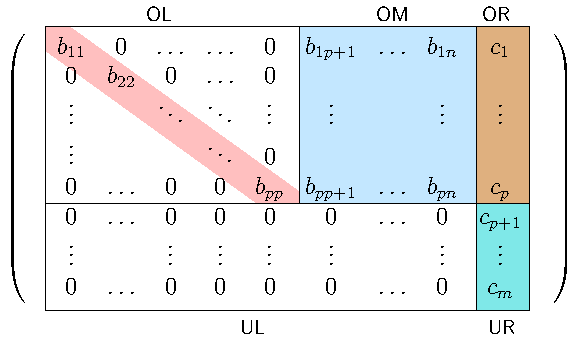
\includegraphics[width=10cm]{LGSDiaMatrix_farb.pdf}
\end{center}
\caption{Die umgeformte erweiterte Koeffizientenmatrix zerfällt in verschiedene Teilmatrizen: \textsf{OL} für ,,oben links'', \textsf{OM} für ,,oben Mitte'' etc.}
\label{fig:LGSDiaMatrix}
\end{figure}

\begin{enumerate}
\item
In Beispiel \ref{Bsp:LGSRosen} wurde gezeigt, wie in der erweiterten Koeffizientenmatrix $(A\mid b)$ Spalten wie in Teil \textsf{OL} in Abbildung \ref{fig:LGSDiaMatrix} gebildet werden können. Voraussetzung war dabei, dass in jeder Spalte $j$ das Element an der Position $j$ ungleich $0$ ist oder an einer rechts unterhalb befindlichen Position ein Element $\neq0$ steht. Ist dies nicht möglich, so bleiben nur noch Zeilen übrig, die, außer in der letzten Spalte, nur $0$ enthalten (Teil \textsf{UL} in Abbildung \ref{fig:LGSDiaMatrix}), die Umwandlung ist dann abgeschlossen.
\item
Wir hatten oben schon plausibel gemacht, dass die Operationen \OP{Ver}-\OP{Add} die Lösungsmenge nicht beeinflussen. Wird \OP{Spa} zur Vertauschung der Spalten $1\le k<l\le n$ verwendet, so müssen bei allen folgenden Überlegungen $x_k$ und $x_l$ vertauscht werden. Dies wird noch einmal unten im Beispiel \ref{Bsp:Kowalski} ausgeführt.
\item
Für $p<m$ haben die letzten $m-p$ Gleichungen des transformierten LGS (**) alle die Gestalt
$$
0\cdot x_1+0\cdot x_2+\cdots +0\cdot x_n = c_k, \quad k=p+1,p+2,\ldots, m.
$$
Gibt es eine Lösung $x$ von $Bx=c$ (und damit von $Ax=b$), so muss dieses $x$ auch die obenstehenden Gleichungen erfüllen, das geht aber nur, wenn $c_{k}=0,k=p+1,\ldots,m$, gilt, wenn also auch im Bereich \textsf{UR} von Abbildung \ref{fig:LGSDiaMatrix} nur $0$ steht. In diesem Falle erfüllt aber jedes $x\in\mathbb R^n$ die letzten $m-p$ Gleichungen. D.\,h.\ umgekehrt, wenn $c_{p+1}=\cdots=c_m=0$ gilt, so entscheidet sich die Frage, ob ein $x\in\mathbb R^n$ eine Lösung ist, nur anhand der ersten $p$ Gleichungen. Das in Teil d) konstruierte $\hat{x}$ zeigt, dass es dann stets eine Lösung von $Bx=c$ (und damit $ Ax=b$) gibt.

Gilt $p=m$, so gibt es keinen Bereich \textsf{UR} und $ \hat{x}$ ist stets eine Lösung.
\item
Ist (*) lösbar und gilt daher $c_{p+1}=\cdots=c_m=0$, so sind die letzten $m-p$ Gleichungen von $Bx=c$ stets erfüllt. Man kann nun ${\hat x}_j:=0$ setzen für $j=p+1,\ldots,n$. Dann  spielen für die Gültigkeit der ersten $p$ Gleichungen die Werte im Bereich \textsf{OM} keine Rolle (da sie mit ${\hat x}_j=0$ multipliziert werden). Die ersten $p$ Gleichungen von (**) werden also von $\hat{x}$ genau dann erfüllt, wenn gilt
$$
\text{\textsf{OL}}\cdot
\begin{pmatrix}
{\hat x}_1\\
{\hat x}_2\\
\vdots\\
{\hat x}_p
\end{pmatrix}
=
\begin{pmatrix}
 c_1\\c_2\\\vdots\\c_p
\end{pmatrix}
$$
also, falls
$$
\begin{pmatrix}
1&0&\cdots & \cdots &0\\
0&1&0&\cdots &0\\
\vdots &&\ddots &\ddots &\vdots\\
\vdots &&&\ddots & 0&\\
0&\cdots &0&0& 1
\end{pmatrix}
\cdot
\begin{pmatrix}
{\hat x}_1\\{\hat x}_2\\\vdots\\{\hat x}_p
\end{pmatrix}
=
\begin{pmatrix}
c_1\\c_2\\\vdots\\c_p
\end{pmatrix}
\quad \text{bzw.}\quad
\begin{aligned}
{\hat x}_1 & = c_1\\
{\hat x}_2 & = c_2\\
\vdots &\quad \vdots\\
{\hat x}_p&=c_p
\end{aligned}\quad.
$$
\end{enumerate}
\end{proof}

Es bleibt noch zu klären, unter welchen Umständen es mehr als eine Lösung gibt und wie diese Lösungen aufzufinden sind. Dazu betrachtet man zunächst anstelle von $Ax=b$ das zugehörige \emph{homogene} LGS $Ax=0$.

\begin{theorem}[LGS-Homogen]\label{Satz:LGShomogen}
Unter den Voraussetzungen wie in Satz \ref{Satz:LGS} gilt:
\begin{enumerate}
\item
$0$ ist immer eine Lösung des homogenen Systems $Ax=0$. Die Lösungsmengen von $ Ax=0$ und $Bx=0$ stimmen überein.
\item
Gilt in \eqref{eq:LGSDiagonalMatrix} $p<n$, so hat das zugehörige homogene LGS $Ax=0$ den Lösungsraum
$$
{\mathbb L}_0:=\big\{\lambda_1 y^{(1)}+ \lambda_2 y^{(2)} +\cdots +\lambda_r y^{(r)} \
\big|\ \lambda_1 ,\ldots,\lambda_r \in\mathbb R\;\big\},
$$
mit $r:=n-p$ und Vektoren $y^{(1)},\ldots,y^{(r)}\in\mathbb R^n,$ wobei
\begin{equation}\label{eq:LGSHomLsg}
y^{(1)}=
\begin{pmatrix}
-b_{1,p+1}\\
-b_{2,p+1}\\
\vdots\\
-b_{p,p+1}\\
\mathbf{1}\\
0\\
\vdots\\
0
\end{pmatrix},\quad
y^{(2)}=
\begin{pmatrix}
-b_{1,p+2}\\
-b_{2,p+2}\\
\vdots\\
-b_{p,p+2}\\
0\\
\mathbf{1}\\
\vdots\\
0
\end{pmatrix},\quad\ldots\quad,
y^{(r)}=
\begin{pmatrix}
-b_{1,n}\\
-b_{2,n}\\
\vdots\\
-b_{p,n}\\
0\\
0\\
\vdots\\
\mathbf{1}
\end{pmatrix},
\end{equation}
dabei sind die $ b_{ij}$ gerade die Werte aus dem Bereich \textsf{OM} in Abbildung \ref{fig:LGSDiaMatrix}. ${\mathbb L}_0$ ist also der von $y^{(1)},\ldots,y^{(r)}$ aufgespannte lineare Unterraum des $\mathbb R^n,$ er hat die Dimension $r=n-p$. Hierbei ist zu berücksichtigen, dass bei einer Verwendung von \OP{SPA} die entsprechenden Komponenten der $y^{(i)}$ umsortiert werden müssen.
\item
Gilt $n=p$ (also $ r=n-p=0$), so hat das homogene System $Ax=0$ \emph{nur} die eine Lösung $x=0$.
\end{enumerate}
\end{theorem}

In Beispiel \ref{Bsp:LGSRosen} galt $n=3=p$, nach Satz \ref{Satz:LGShomogen} b) folgt also, dass $x:=0$ die einzige Lösung des homogenen LGS $Ax=0$ ist. Es gibt also keine Aufteilung für die Blumen, die $ 0$ Fläche einnimmt, $0$ Euro kostet und kein Düngemittel braucht, es sei denn, man lässt es ganz. Dies ist nicht so selbstverständlich, denn es könnten durchaus Lösungen mit negativen Komponenten existieren, die sich z.\,B.\ zur ,,Fläche'' $0$ addieren. Dies wäre natürlich keine Lösung, die sich realisieren ließe, da es keine negativen Anbauflächen gibt. Wir haben oben Glück gehabt, dass die gefundene Lösung eine Nebenbedingung erfüllt, die wir nicht genannt haben: alle $x_i$ müssen $\ge 0$ sein.

\begin{proof}[Beweis zu Satz LGS-Homogen]
\begin{enumerate}
\item
Zum homogenen LGS $Ax=0$ gehört das transformierte homogene LGS $Bx=0$. Wir zeigen, dass $y^{(1)},\ldots,y^{(r)}$ Lösungen davon sind. Die $i$-te Gleichung ($1\le i\le p$) von $By^{(l)}=0$ hat wegen \eqref{eq:LGSHomLsg} die Gestalt
\begin{equation}\label{eq:Hom1}
\sum_{j=1}^nb_{ij}y_j^{(l)}=1\cdot y_i^{(l)}+\sum_{j=p+1}^n b_{ij}y_j^{(l)}= 1\cdot( -b_{i,p+l})+ b_{i,p+l}\cdot 1 =0.
\end{equation}
Also erfüllen die $y^{(l)}$ das homogene LGS $ Ax=0$ (eventuell nach Umsortieren der Koordinaten bei Anwendung von Spaltentausch \OP{Spa}). Damit
erfüllen aber auch alle Linearkombinationen $\lambda_1 y^{(1)}+\cdots+\lambda_r y^{(r)}$ dieses System, denn es gilt für beliebige $\lambda_1,\ldots,\lambda_r \in\mathbb R$
\[
A(\lambda_1 y^{(1)}+\cdots+\lambda_r y^{(r)})= \lambda_1 Ay^{(1)}+\cdots+\lambda_rA y^{(r)}=\lambda_10 +\cdots+\lambda_r0=0.
\]
Die Gestalt der letzten $r$ Komponenten von $y^{(1)} ,\ldots,y^{(r)}$ (jeweils genau eine ,,$1$'' an jeweils einer anderen Stelle) zeigt, dass diese Lösungen linear unabhängig sind. ${\mathbb L}_0$ hat also mindestens die Dimension $r$. Man kann zeigen, dass ${\mathbb L}_0$  auch genau diese Dimension hat.  Daher bilden $y^{(1)},\ldots,y^{(r)}$ eine Basis von ${\mathbb L}_0$, jede Lösung lässt sich daher als eine Linearkombination aus $y^{(1)} ,\ldots,y^{(r)}$ darstellen.
\item
$A0=0$ gilt offensichtlich für alle Matrizen $A$, daher ist $x:=0$ immer eine Lösung des homogenen LGS. Für $n=p$ gibt es keine Vektoren $y^{(l)}$, es kann daher keine weitere Lösung geben.
\end{enumerate}
\end{proof}

Aus den beiden vorangegangenen Sätzen lässt sich nun die genaue Gestalt der Lösungsmenge $\mathbb L$ des ursprünglichen LGS gewinnen. Dabei macht man sich folgende Überlegung zu Nutze: hat man eine Lösung $\hat{x}$ des LGS $Ax=b$ (wie z.\,B.\ in Satz \ref{Satz:LGS} d)), so kann man immer eine Lösung $y$ des homogenen Systems dazuaddieren und erhält wieder eine Lösung von $Ax=b$, denn es gilt
\begin{equation}\label{eq:zusgLsg}
A(\hat{x}+y)= A\hat{x}+Ay=a\hat{x}=b
\end{equation}
wegen $Ay=0$.

\begin{theorem}[LGS-allgemeiner Fall]\label{Satz:LGSallg}
Unter den Voraussetzungen des Satzes \ref{Satz:LGS} gilt:
\begin{enumerate}
\item
Ist (*) lösbar, so haben die Lösungen die Gestalt
$$
{\hat x}+y,\quad \text{ mit } y \in {\mathbb L}_0,
$$
d.\,h., jede Lösung $x$ von \eqref{eq:LGS1} ist darstellbar als Summe aus der speziellen Lösung ${\hat x}$ aus Satz \ref{Satz:LGS} d) und einer Lösung des homogenen Systems $ Ax=0,$ also als
\begin{equation}\label{eq:LGSalgLsg}
x = \hat{x} + \lambda_1 y^{(1)}+\cdots + \lambda_r y^{(r)}
\end{equation}
für $\lambda_1,\ldots, \lambda_r\in\mathbb R$ und $y^{(1)},\ldots, y^{(r)}$ aus \eqref{eq:LGSHomLsg}.
\item
Ist (*) lösbar mit $p=n$ (und daher $r=0$), so ist ${\hat x}$ aus Satz \ref{Satz:LGS} d) die einzige Lösung von \eqref{eq:LGS1}.
\end{enumerate}
\end{theorem}

Im Beispiel \ref{Bsp:LGSRosen} galt $p=n=3$, die einzige Lösung des homogenen Systems war $x=0$, daher ist die Lösung $ \hat{x}^T=(120,370,10)$ die einzige Lösung des Systems.

Die drei Sätze \ref{Satz:LGS}, \ref{Satz:LGShomogen} und \ref{Satz:LGSallg} besagen zusammengenommen, dass die Lösung linearer Gleichungssysteme im
Wesentlichen auf folgenden Punkten beruht:
\begin{itemize}
\item
Umwandlung der erweiterten Koeffizientenmatrix in eine einfache Normgestalt \eqref{eq:LGSDiagonalMatrix},
\item
direktes Ablesen der Lösbarkeit an dieser Gestalt (Satz \ref{Satz:LGS} c)),
\item
gegebenenfalls direktes Ablesen einer speziellen Lösung (Satz \ref{Satz:LGS} d)),
\item
Beschreibung weiterer Lösungen mithilfe des homogenen LGS (Satz \ref{Satz:LGSallg} a)).
\end{itemize}

\begin{proof}[Beweis zu Satz LGS-allgemeiner Fall]
In \eqref{eq:zusgLsg} hatten wir bereits gezeigt, dass für $y\in{\mathbb L}_0$
$$
\bar{x}:={\hat x}+y
$$
eine Lösung von (*) ist. Ist umgekehrt $x$ irgendeine Lösung von (*), so ist ${\tilde x}:=x-{\hat x}$ eine Lösung des homogenen Systems, denn es gilt
$$
A{\tilde x}=A(x-{\hat x})=Ax-A{\hat x}=b-b=0.
$$
Also hat $x ={\hat x}+{\tilde x}$ die gewünschte Gestalt.
\end{proof}


\begin{example}\label{Bsp:Kowalski}
Es soll das folgende LGS untersucht werden:
\begin{alignat*}{4}
x_1&\ +\ &3x_2&\ -\ &4x_3&\ +\ &3x_4&=9\\
3x_1&\ +\ &9x_2&\ -\ &2x_3&\ -\ &11x_4&=\ -\ 3\\
4x_1&\ +\ &12x_2&\ -\ &6x_3&\ -\ &8x_4&=6\\
2x_1&\ +\ &6x_2&\ +\ &2x_3&\ -\ &14x_4&=-12\ ,
\end{alignat*}
dazu gehört die erweiterte Koeffizientenmatrix
$$
(A\mid b)=\left(\begin{array}{cccc|c}
1&3&-4&3&9\\
3&9&-2&-11&-3\\
4&12&-6&-8&6\\
2&6&2&-14&-12
\end{array}\right).
$$
Um das Vertauschen von Spalten nach Operation \OP{Spa} nachverfolgen zu können, fügen wir noch eine erste Zeile mit den Spaltennummern ($=$Indizes
der Lösungsvariablen $x_i$) hinzu.

Durch Subtraktion des entsprechenden ($ a_{i1}$-fachen) Vielfachen der ersten Zeile von allen anderen erhält man:
$$
\begin{pmatrix}
_1&_2&_3&_4&\\
{1}&3&-4&3&\Big |& 9\\
{0}&0&10&-20&\Big |&-30\\
{0}&0&10&-20&\Big |&-30\\
{0}&0&10&-20&\Big | &-30
\end{pmatrix}
$$
Damit ist Spalte $1$ abgearbeitet. In Spalte $j=2$ steht an Position $2$ eine $0$, daher tauschen wir die zweite und dritte Spalte aus, und erhalten:
$$
\begin{pmatrix}
_1&_3&_2&_4&\\
1 &-4&3 &3&\Big |& 9\\
0 &10&0 &-20&\Big |&-30\\
0 &10&0 &-20&\Big |&-30\\
0 &10&0 &-20&\Big | &-30
\end{pmatrix}
$$
Die zweite Spalte hat jetzt an Position $2$ den Wert $10\neq0$, wir können sie daher durch $10$ teilen und entsprechende Vielfache (hier das $10$-fache) von den darunterliegenden Zeilen abziehen. Wir erhalten dann:
$$
\begin{pmatrix}
_1&_\mathbf{3}&_\mathbf{2}&_4&&\\
1&-4&3&3&\Big |&9\\
0&1&0&-2&\Big |&-3\\
0&0&0&0&\Big |&0\\
0&0&0&0&\Big |&0
\end{pmatrix}
$$
Um die Bearbeitung von Spalte $2$ abzuschließen, addieren wir noch das $4$-fache der zweiten Zeile zur ersten und erhalten:
$$
\left(B\mid c\right)=
\begin{pmatrix}
_1&_3&_2&_4&&\\
1&0&3&-5&\Big |&-3\\
0&1&0&-2&\Big | &-3\\
0&0&\GB{0}&\GB{0}&\Big |&0\\
0&0&\GB{0}&\GB{0}&\Big |&0
\end{pmatrix}
$$
In der dritten Spalte steht in der dritten Zeile eine $0$ und auch alle anderen Werte rechts unterhalb davon sind $0$. Die Transformation ist damit abgeschlossen, die Matrix hat jetzt die Gestalt wie in Abbildung \ref{fig:LGSDiaMatrix} bzw.\ \eqref{eq:LGSDiagonalMatrix} mit $n=m=4$ und $p=2$.

Es gilt $c_3=c_4=0$, also ist das LGS nach Satz \ref{Satz:LGS} c) lösbar.

Eine spezielle Lösung ${\tilde x}$ des inhomogenen Systems $Bx=b$ ist nach Satz \ref{Satz:LGS} d)
$$
{\tilde x}\ =\
\begin{pmatrix}c_1\\c_2\\0\\0\end{pmatrix}
\ =\
\begin{pmatrix}-3\\ -3\\ 0\\0\end{pmatrix}
\ =\
\begin{pmatrix}\tilde{x}_1\\\tilde{x}_2\\\tilde{x}_3\\\tilde{x}_4\end{pmatrix}.
$$
Hier ist nun  zu berücksichtigen, dass die 2.\ und 3.\ Spalte von $A$ beim Übergang zu $B$ oben vertauscht wurden. Diese Spalten beziehen sich auf die 2.\ und 3.\ Komponente der Lösungsvektoren. Um zu einer Lösung von $Ax=b$ zu gelangen, muss in ${\tilde x}$ die Vertauschung der 2.\ und 3.\ Spalte rückgängig gemacht werden, also ist
$$
{\hat x} :=\
\begin{pmatrix}-3\\0\\-3\\0\end{pmatrix}
\ =\
\begin{pmatrix}\hat{x}_1\\\hat{x}_2\\\hat{x}_3\\\hat{x}_4\end{pmatrix}
$$
eine Lösung von $Ax=b$.

Aus Satz \ref{Satz:LGShomogen} a) folgt, dass der Lösungsraum ${\mathbb L}_0$ des homogenen Systems $Ax=0$ die Dimension $r=n-p=2$ hat. Die beiden Vektoren, die den Lösungsraum ${\mathbb L}_0$ von $ Bx=0$ aufspannen, haben nach (\ref{eq:LGSHomLsg}) zunächst die Gestalt
$$
{\tilde y}^{(1)}
:=
\begin{pmatrix}-b_{1,p+1}\\-b_{2,p+1}\\1\\0\end{pmatrix}
=
\begin{pmatrix}-3\\ 0\\ 1\\ 0\end{pmatrix},
\quad
{\tilde y}^{(2)}
:=
\begin{pmatrix}-b_{1,p+2}\\-b_{2,p+2}\\0\\1\end{pmatrix}
=
\begin{pmatrix}5\\2\\0\\1\end{pmatrix}.
$$
Um zu Lösungen des ursprünglichen homogenen Systems $Ax=0$ zu kommen, müssen wir auch in den Vektoren $\tilde{y}^{(1)}$ und $\tilde{y}^{(2)}$ die Komponenten 2 und 3 wieder zurücktauschen und erhalten
$$
y^{(1)}:=\begin{pmatrix}-3\\1\\0\\0\end{pmatrix},\quad
y^{(2)}:=\begin{pmatrix}5\\0\\2\\1\end{pmatrix}.
$$
Die Lösungen des homogenen Systems $Ax=0$ sind also genau die Linearkombinationen aus diesen beiden Vektoren:
\[
\lambda_1\begin{pmatrix}-3\\1\\0\\0\end{pmatrix}+
\lambda_2\begin{pmatrix}5\\0\\2\\1\end{pmatrix} \ =\
\begin{pmatrix}-3\lambda_1+5\lambda_2\\\lambda_1\\2\lambda_2\\\lambda_2\end{pmatrix}
\]
für $\lambda_1,\lambda_2\in\mathbb R$. Die allgemeine Lösung von $Ax=b$ (d.\,h.\ die Elemente von ${\mathbb L}={\hat x}+{\mathbb L}_0$) lässt sich nach Satz \ref{Satz:LGSallg}  also schreiben als
$$
{\hat x}+\lambda_1 y^{(1)}+\lambda_2 y^{(2)}=
\begin{pmatrix}
-3-3\lambda_1+5\lambda_2\\
\lambda_1\\
-3+2\lambda_2\\
\lambda_2
\end{pmatrix}
$$
für $\lambda_1,\lambda_2\in\mathbb R$.
\end{example}

\begin{example}\label{Bsp:RosenNelkenUnloesbar}
\begin{enumerate}
\item
Wir betrachten noch einmal das Gärtnerbeispiel \ref{Bsp:RosenNelken}, nehmen jetzt aber an, dass der Verbrauch des Düngemittels II pro m$^2$ für alle Pflanzen lediglich $1$ kg beträgt (gegenüber $2$ kg oben). Dann erhalten wir das LGS
\begin{alignat}{4}
x_1&\ +\ &x_2&\ +\ &x_3&=500 \tag{\RM{1}}\\
3x_1&\ +\ &7x_2&\ +\ &5x_3&=3000 \tag{\RM{2}}\\
x_1&\ +\ &2x_2&\ +\ &3x_3&=890 \tag{\RM{3}}\\
x_1&\ +\ &x_2&\ +\ &x_3&=1000 \tag{\RM{4}}
\end{alignat}
mit der erweiterten Koeffizientenmatrix
$$
(A\mid b)=\left(\begin{array}{ccc|c}
1&1&1&500\\
3&7&5&3000\\
1&2&3&890\\
1&1&1&1000
\end{array}\right).
$$
Dieselben Schritte wie in Beispiel \ref{Bsp:LGSRosen} führen nacheinander zu den folgenden Matrizen:
\begin{eqnarray*}
\left(\begin{array}{ccc|c}
1&1&1&500\\
3&7&5&3000\\
1&2&3&890\\
1&1&1&1000
\end{array}\right)\stackrel{\text{\OP{Add}}}{\Rightarrow}
\left(\begin{array}{ccc|c}
1&1&1&500\\
0&4&2&1500\\
0&1&2&390\\
0&0&0&500
\end{array}\right)\stackrel{\text{\OP{Mul}}}{\Rightarrow}
\left(\begin{array}{ccc|c}
1&1&1&500\\
0&1&1/2&375\\
0&1&2&390\\
0&0&0&500
\end{array}\right)
\\
\stackrel{\text{\OP{Add}}}{\Rightarrow}
\left(\begin{array}{ccc|c}
1&0&1/2&125\\
0&1&1/2&375\\
0&0&3/2&15\\
0&0&0&500
\end{array}\right)\stackrel{\text{\OP{Mul}}}{\Rightarrow}
\left(\begin{array}{ccc|c}
1&0&1/2&125\\
0&1&1/2&375\\
0&0&1&10\\
0&0&0&500
\end{array}\right)\stackrel{\text{\OP{Add}}}{\Rightarrow}
\left(\begin{array}{ccc|c}
1&0&0&120\\
0&1&0&370\\
0&0&1&10\\
0&0&0&500
\end{array}\right)
\end{eqnarray*}
Dies ist die Gestalt aus \eqref{eq:LGSDiagonalMatrix} mit $n=p=3$, hier gilt aber $c_{p+1}=c_4=500\neq0$. Das System ist also nicht lösbar. Dies wird
anschaulich daraus klar, dass die erste Gleichung verlangt, dass sich $x_1,x_2,x_3$ zu (der Fläche) $500$ aufaddieren, in der letzten Gleichung aber
wird verlangt, dass dieselbe Summe $1000$ (Düngemittel II) ergibt. Im LGS steckt also ein Widerspruch.
\item
Ändert man in dem ursprünglichen Beispiel die dritte Gleichung in
\[
1.5 x_1 + 3.5 x_2+2.5 x_3 = 1500
\]
so erhält man folgende Umformungen:
\begin{eqnarray*}
\left(\begin{array}{ccc|c}
1&1&1&500\\
3&7&5&3000\\
1.5&3.5&2.5&1500\\
2&2&2&1000
\end{array}\right)&\stackrel{\text{\OP{Add}}}{\Rightarrow}&
\left(\begin{array}{ccc|c}
1&1&1&500\\
0&4&2&1500\\
0&2&1&750\\
0&0&0&0
\end{array}\right)\stackrel{\text{\OP{Mul}}}{\Rightarrow}
\left(\begin{array}{ccc|c}
1&1&1&500\\
0&1&1/2&375\\
0&2&1&750\\
0&0&0&0
\end{array}\right)\\
&\stackrel{\text{\OP{Add}}}{\Rightarrow}&
\left(\begin{array}{ccc|c}
1&0&1/2&125\\
0&1&1/2&375\\
0&0&0&0\\
0&0&0&0
\end{array}\right)
\end{eqnarray*}
Hier wurde im letzten Schritt das $2$-fache der zweiten Zeile von der dritten abgezogen. Damit ist die Gestalt aus \eqref{eq:LGSDiagonalMatrix} erreicht, hier mit $n=3$, $m=4$, $p=2$. Das System ist lösbar wegen $c_3=c_4=0$. Die spezielle Lösung lautet nach Satz \ref{Satz:LGS} d)
\[
\hat{x}=\begin{pmatrix}125\\375\\0\end{pmatrix},
\]
es werden also keine Nelken angebaut. Das homogene LGS hat nach Satz \ref{Satz:LGShomogen} mit $r:=n-p=3-2=1$ einen Lösungsraum ${\mathbb L}_0$ der Dimension $1$, der nach \eqref{eq:LGSHomLsg} von dem Basisvektor ($p=2$!)
\[
y^{(1)}=
\begin{pmatrix}-b_{1,p+1}\\ -b_{2,p+1}\\ \vdots\\ -b_{p,p+1}\\ 1\\ 0\\ \vdots\\ 0\end{pmatrix}=
\begin{pmatrix}-b_{13}\\-b_{23}\\1\end{pmatrix}=
\begin{pmatrix}-\frac{1}{2}\\-\frac{1}{2}\\1\end{pmatrix}
\]
aufgespannt wird. Der Lösungsraum hat also die Gestalt
\[
{\mathbb L}_0=\Big\{ \lambda \cdot \begin{pmatrix}-1/2\\-1/2\\1\end{pmatrix}\mid \lambda \in\mathbb R\Big\}.
\]
Setzt man $\beta=1/2\lambda$, so erhält man die etwas einfachere Gestalt
\[
{\mathbb L}_0= \Big\{ \beta \cdot \begin{pmatrix}-1\\-1\\2\end{pmatrix}\mid \beta \in\mathbb R\Big\}.
\]
Die Lösungen des ursprünglichen Systems haben also die Gestalt:
\[
\hat{x}+\beta\begin{pmatrix}-1\\-1\\2\end{pmatrix}=
\begin{pmatrix}125-\beta\\375-\beta\\2\beta\end{pmatrix},\quad \beta\in\mathbb R.
\]
So sind z.\,B.\ für $\beta=10$ bzw.\ $\beta=125$
\[
\begin{pmatrix}115\\365\\20\end{pmatrix} ~\text{bzw.}~ \begin{pmatrix}0\\250\\250\end{pmatrix}
\]
Lösungen. Für $\beta>125$ erhält man Lösungen, die rechnerisch das LGS lösen, aber nicht als Flächenanteile realisierbar sind, da sie negative Komponenten enthalten, z.\,B.
\[
\begin{pmatrix}-25\\225\\300\end{pmatrix} \quad ~\text{für}~ \beta=150.
\]
Etwas Ähnliches passiert für $\beta<0$.
\end{enumerate}
\end{example}

Die in (\ref{eq:LGSDiagonalMatrix}) beschriebene Form der transformierten Matrix ist der allgemeine Fall mit $p\le\min\{m,n\}$. Es können auch folgende Spezialfälle davon auftreten.

\begin{itemize}
\item
\textbf{Fall 1}: Gilt $p=m<n$, so hat die Zielmatrix folgende Gestalt
\begin{equation*}
(B\mid c)=
\left(\begin{array}{cccccccc|c}
1&0&\cdots&\cdots&0&b_{1p+1}&\cdots&b_{1n}&c_1\\
0&1&0&\cdots&0&&&&c_2\\
\vdots&0&\ddots&\ddots&\vdots&\vdots&&\vdots&\vdots\\
\vdots&\vdots&\ddots&\ddots&0&\vdots&&\vdots&\vdots\\
0&0&\cdots&0&1&b_{pp+1}&\cdots&b_{pn}&c_p
\end{array}\right)
\end{equation*}
Da es keine $c_{p+1},\ldots,c_n$ gibt, ist ein solches System nach Satz \ref{Satz:LGS} c) \emph{immer lösbar}.
\item
\textbf{Fall 2}: Für den wichtigen Fall $p=m=n$ erhält man
\begin{equation*}
(B\mid c)=
\left(\begin{array}{ccccc|c}
1&0&\cdots&\cdots&0&c_1\\
0&1&0&\cdots&0&c_2\\
\vdots&0&\ddots&\ddots&\vdots&\vdots\\
\vdots&&\ddots&\ddots&0&\vdots\\
0&0&\cdots&0&1&c_p
\end{array}\right),
\end{equation*}
und für $p=n<m$
\begin{equation*}
(B\mid c)=
\left(\begin{array}{ccccc|c}
1&0&\cdots&\cdots&0&c_1\\
0&1&0&\cdots&0&c_2\\
\vdots&0&\ddots&\ddots&\vdots&\vdots\\
\vdots&&\ddots&\ddots&0&\vdots\\
0&0&\cdots&0&1&c_p\\
0&\cdots&0&0&0&c_{p+1}\\
\vdots&&&&\vdots&\vdots\\
0&\cdots&0&0&0&c_m
\end{array}\right).
\end{equation*}
\end{itemize}

\end{document}